\newpage
\subsection{Caso d'uso UC12: Risposta ad una domanda}
\label{UC12}
\begin{figure}[h]
	\centering
	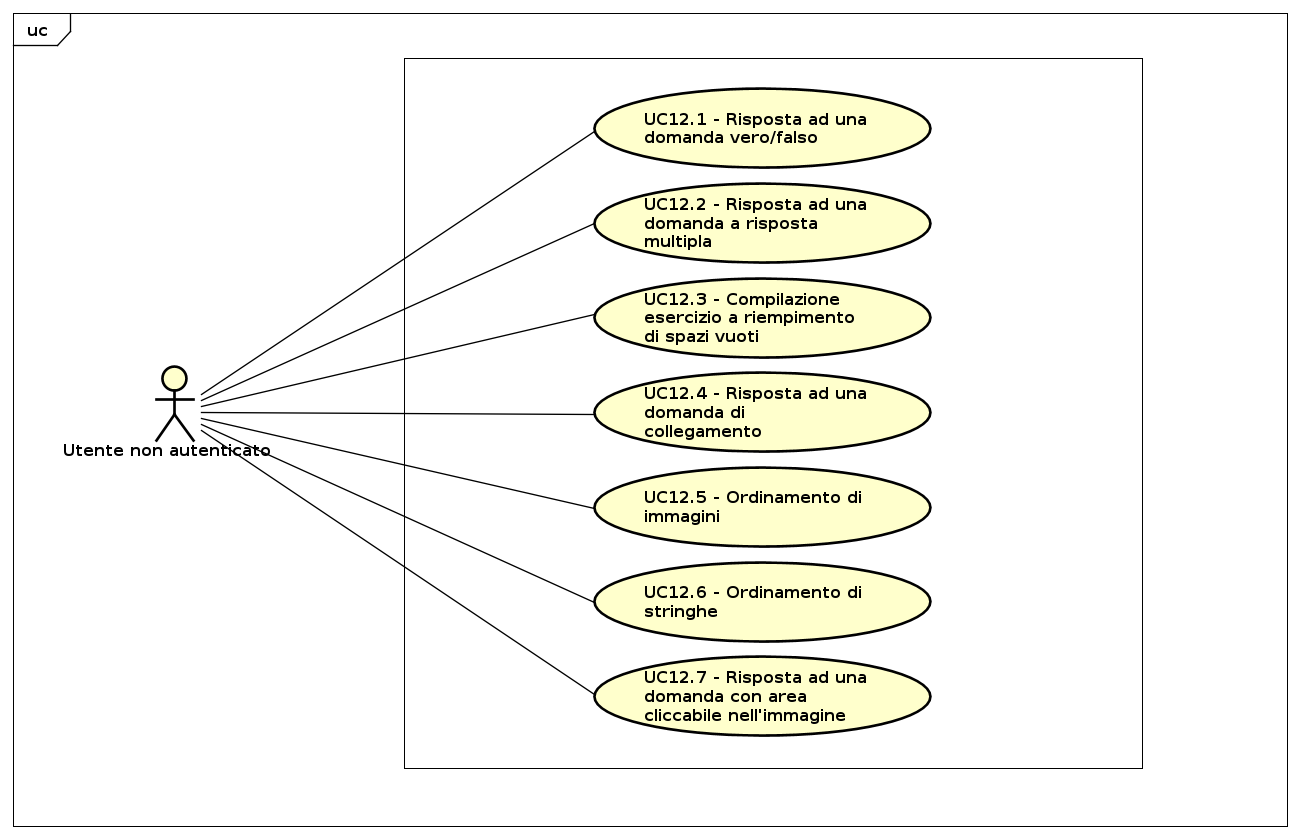
\includegraphics[scale=0.5]{UML/UC12.png}
	\caption{UC12: Risposta ad una domanda}
\end{figure}

\begin{itemize}
\item \textbf{Attori}: utente autenticato, utente autenticato pro;
\item \textbf{Descrizione}: l'attore può rispondere alla domanda che viene visualizzata selezionando una o più risposte proposte, riempiendo gli spazi vuoti, ordinando le risposte oppure associando due voci;
\item \textbf{Precondizione}: l'attore visualizza la domanda e le possibili risposte;
\item \textbf{Postcondizione}: l'attore ha selezionato una o più risposte;
\item \textbf{Scenario principale}: si verifica uno dei seguenti scenari:
\begin{enumerate}
	\item L'attore risponde ad una domanda vero/falso (UC12.1);
	\item L'attore risponde ad una domanda con risposte multiple (UC12.2);
	\item L'attore compila un esercizio riempiendo gli spazi vuoti (UC12.3);
	\item L'attore associa le voci della colonna di sinistra con quelle della colonna di destra (UC12.4);
	\item L'attore ordina le immagini secondo il criterio richiesto dalla domanda (UC12.5);
	\item L'attore ordina le stringhe secondo il criterio richiesto dalla domanda (UC12.6);
	\item L'attore risponde alla domanda selezionando un'area cliccabile (UC12.7). 
\end{enumerate}
\end{itemize}

\subsubsection{Caso d'uso UC12.1: Risposta ad una domanda vero/falso}
\begin{itemize}
\item \textbf{Attori}: utente autenticato, utente autenticato pro;
\item \textbf{Descrizione}: l'attore può selezionare una risposta alla domanda vero/falso;
\item \textbf{Precondizione}: l'attore visualizza la domanda vero/falso;
\item \textbf{Postcondizione}: l'attore ha risposto alla domanda vero/falso;
\item \textbf{Scenario principale}: l'attore seleziona una risposta alla domanda vero/falso.
\end{itemize}

\subsubsection{Caso d'uso UC12.2: Risposta ad una domanda a risposta multipla}
\begin{itemize}
\item \textbf{Attori}: utente autenticato, utente autenticato pro;
\item \textbf{Descrizione}: l'attore può selezionare una o più risposte alla domanda a risposta multipla;
\item \textbf{Precondizione}: l'attore visualizza la domanda a risposta multipla;
\item \textbf{Postcondizione}: l'attore ha risposto alla domanda a risposta multipla;
\item \textbf{Scenario principale}: l'attore seleziona una o più risposte alla domanda a risposta multipla.
\end{itemize}

\subsubsection{Caso d'uso UC12.3: Compilazione esercizio di riempimento degli spazi vuoti}
\begin{figure}[h]
	\centering
	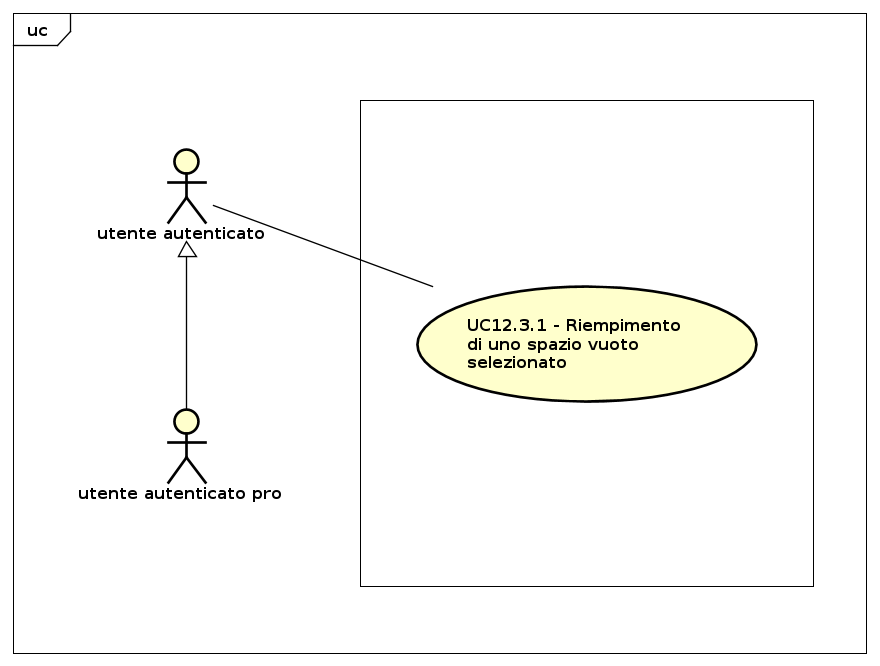
\includegraphics[scale=0.5]{UML/UC12_3.png}
	\caption{UC12.3: Compilazione esercizio di riempimento degli spazi vuoti}
\end{figure}
\begin{itemize}
\item \textbf{Attori}: utente autenticato, utente autenticato pro;
\item \textbf{Descrizione}: l'attore può compilare l'esercizio riempiendone gli spazi;
\item \textbf{Precondizione}: l'attore visualizza l'esercizio di riempimento degli spazi vuoti;
\item \textbf{Postcondizione}: l'attore ha compilato l'esercizio riempiendone gli spazi;
\item \textbf{Scenario principale}: l'attore compila l'esercizio riempiendone gli spazi  (UC12.3.1).
\end{itemize}

\paragraph{Caso d'uso UC12.3.1: Riempimento di uno spazio vuoto selezionato}
\begin{itemize}
\item \textbf{Attori}: utente autenticato, utente autenticato pro;
\item \textbf{Descrizione}: l'attore può riempire o modificare lo spazio selezionato;
\item \textbf{Precondizione}: l'attore ha selezionato uno spazio;
\item \textbf{Postcondizione}: l'attore ha riempito lo spazio selezionato;
\item \textbf{Scenario principale}: l'attore riempie o modifica lo spazio selezionato;
\item \textbf{Scenario alternativo}: l'attore seleziona un altro spazio per riempirlo o modificarlo. 
\end{itemize}

\subsubsection{Caso d'uso UC12.4: Risposta ad una domanda di collegamento}
\begin{figure}[h]
	\centering
	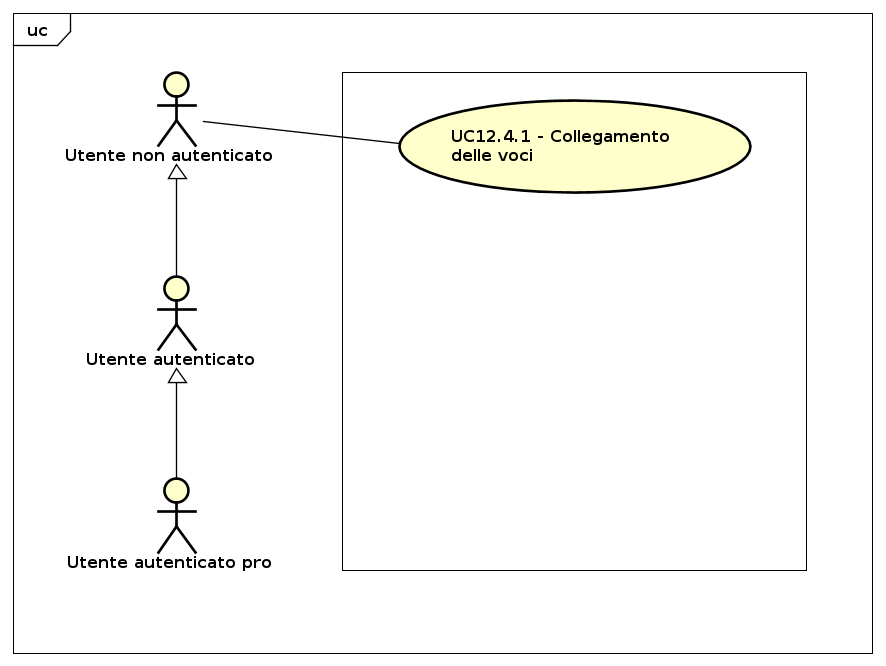
\includegraphics[scale=0.5]{UML/UC12_4.png}
	\caption{UC12.4: Risposta ad una domanda di collegamento}
\end{figure}
\begin{itemize}
\item \textbf{Attori}: utente autenticato, utente autenticato pro;
\item \textbf{Descrizione}: l'attore può collegare le voci della colonna di sinistra con le voci della colonna di destra;
\item \textbf{Precondizione}: l'attore visualizza la domanda di collegamento;
\item \textbf{Postcondizione}: l'attore ha collegato le voci della colonna di sinistra con le voci della colonna di destra;
\item \textbf{Scenario principale}: l'attore collega le voci della colonna di sinistra con le voci della colonna di destra (UC12.4.1).
\end{itemize}

\newpage
\paragraph{Caso d'uso UC12.4.1: Collegamento delle voci}
\begin{figure}[h]
	\centering
	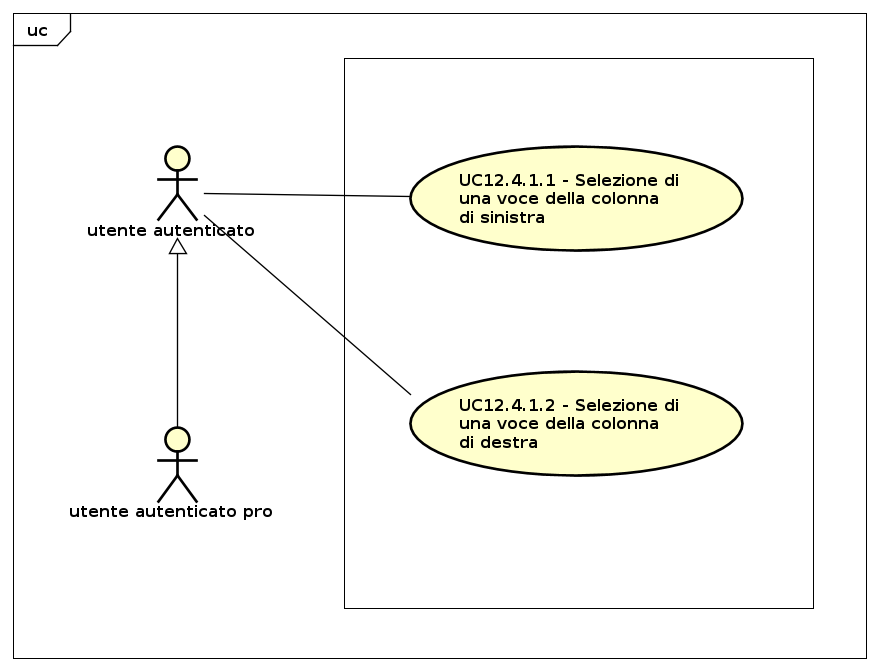
\includegraphics[scale=0.5]{UML/UC12_4_1.png}
	\caption{UC12.4.1: Collegamento delle voci}
\end{figure}
\begin{itemize}
\item \textbf{Attori}: utente autenticato, utente autenticato pro;
\item \textbf{Descrizione}: l'attore può selezionare una voce della colonna di sinistra/destra e successivamente selezionare una voce della colonna di destra/sinistra per associarle;
\item \textbf{Precondizione}: l'attore visualizza le colonne con le voci da associare;
\item \textbf{Postcondizione}: l'attore ha associato due voci;
\item \textbf{Scenario principale}: l'attore seleziona una voce della colonna di sinistra/destra (UC12.4.1.1)/(UC12.4.1.2) e successivamente seleziona una voce della colonna di destra/sinistra per associarle.
\end{itemize}

\subparagraph{Caso d'uso UC12.4.1.1: Selezione di una voce della colonna di sinistra}
\begin{itemize}
\item \textbf{Attori}: utente autenticato, utente autenticato pro;
\item \textbf{Descrizione}: l'attore può selezionare una voce della colonna di sinistra;
\item \textbf{Precondizione}: l'attore visualizza le voci della colonna di sinistra;
\item \textbf{Postcondizione}: l'attore ha selezionato una voce della colonna di sinistra;
\item \textbf{Scenario principale}: l'attore seleziona una voce della colonna di sinistra. 
\end{itemize}

\subparagraph{Caso d'uso UC12.4.1.2: Selezione di una voce della colonna di destra}
\begin{itemize}
\item \textbf{Attori}: utente autenticato, utente autenticato pro;
\item \textbf{Descrizione}: l'attore può selezionare una voce della colonna di destra;
\item \textbf{Precondizione}: l'attore visualizza le voci della colonna di destra;
\item \textbf{Postcondizione}: l'attore ha selezionato una voce della colonna di destra;
\item \textbf{Scenario principale}: l'attore seleziona una voce della colonna di destra. 
\end{itemize}

\subsubsection{Caso d'uso UC12.5: Ordinamento di immagini}
\begin{figure}[h]
	\centering
	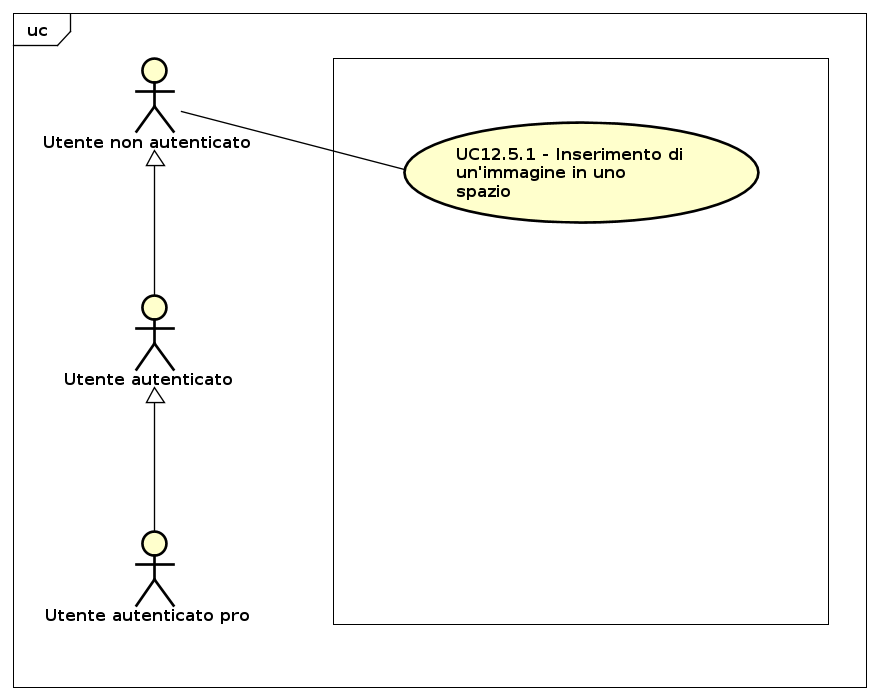
\includegraphics[scale=0.5]{UML/UC12_5.png}
	\caption{UC12.5: Ordinamento di immagini}
\end{figure}
\begin{itemize}
\item \textbf{Attori}: utente autenticato, utente autenticato pro;
\item \textbf{Descrizione}: l'attore può ordinare le immagini secondo il criterio richiesto nella domanda inserendole negli appositi spazi;
\item \textbf{Precondizione}: l'attore visualizza la lista non ordinata delle immagini e la lista vuota in cui andranno inserite;
\item \textbf{Postcondizione}: l'attore ha inserito le immagini nella lista ordinata;
\item \textbf{Scenario principale}: l'attore ordina le immagini secondo il criterio richiesto nella domanda inserendole negli appositi spazi (UC12.5.1).
\end{itemize}

\newpage
\paragraph{Caso d'uso UC12.5.1: Inserimento di un'immagine in uno spazio}
\begin{figure}[h]
	\centering
	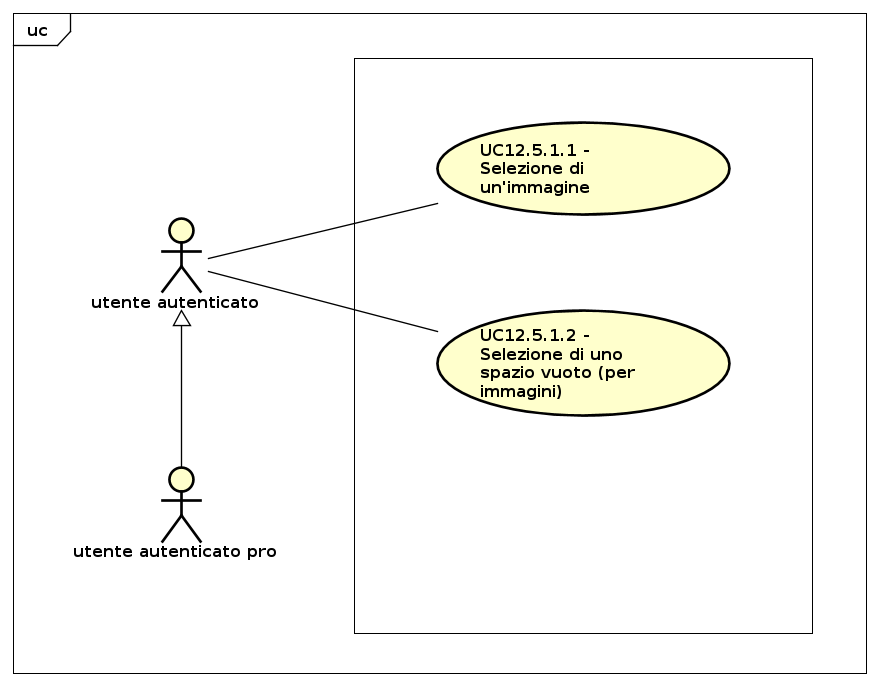
\includegraphics[scale=0.5]{UML/UC12_5_1.png}
	\caption{UC12.5.1: Inserimento di un'immagine in uno spazio}
\end{figure}
\begin{itemize}
\item \textbf{Attori}: utente autenticato, utente autenticato pro;
\item \textbf{Descrizione}: l'attore può selezionare un'immagine per inserirla in uno spazio vuoto o scambiarla con un'altra se lo spazio è già occupato;
\item \textbf{Precondizione}: l'attore visualizza le immagini non ordinate e gli spazi vuoti;
\item \textbf{Postcondizione}: l'attore ha inserito l'immagine nello spazio selezionato;
\item \textbf{Scenario principale}: l'attore seleziona un'immagine (UC12.5.1.1) e la inserisce in uno spazio vuoto o la scambia con un'altra se lo spazio è già occupato (UC12.5.1.2).
\end{itemize}

\subparagraph{Caso d'uso UC12.5.1.1: Selezione di un'immagine}
\begin{itemize}
\item \textbf{Attori}: utente autenticato, utente autenticato pro;
\item \textbf{Descrizione}: l'attore può selezionare un'immagine;
\item \textbf{Precondizione}: l'attore visualizza le immagini non ordinate e gli spazi vuoti;
\item \textbf{Postcondizione}: l'attore ha selezionato un'immagine;
\item \textbf{Scenario principale}: l'attore seleziona un'immagine.
\end{itemize}

\subparagraph{Caso d'uso UC12.5.1.2: Selezione di uno spazio vuoto (per immagini)}
\begin{itemize}
\item \textbf{Attori}: utente autenticato, utente autenticato pro;
\item \textbf{Descrizione}: l'attore può selezionare uno spazio vuoto;
\item \textbf{Precondizione}: l'attore visualizza le immagini non ordinate e gli spazi vuoti;
\item \textbf{Postcondizione}: l'attore ha selezionato uno spazio vuoto;
\item \textbf{Scenario principale}: l'attore seleziona uno spazio vuoto.
\end{itemize}

\subsubsection{Caso d'uso UC12.6: Ordinamento di stringhe}
\begin{figure}[h]
	\centering
	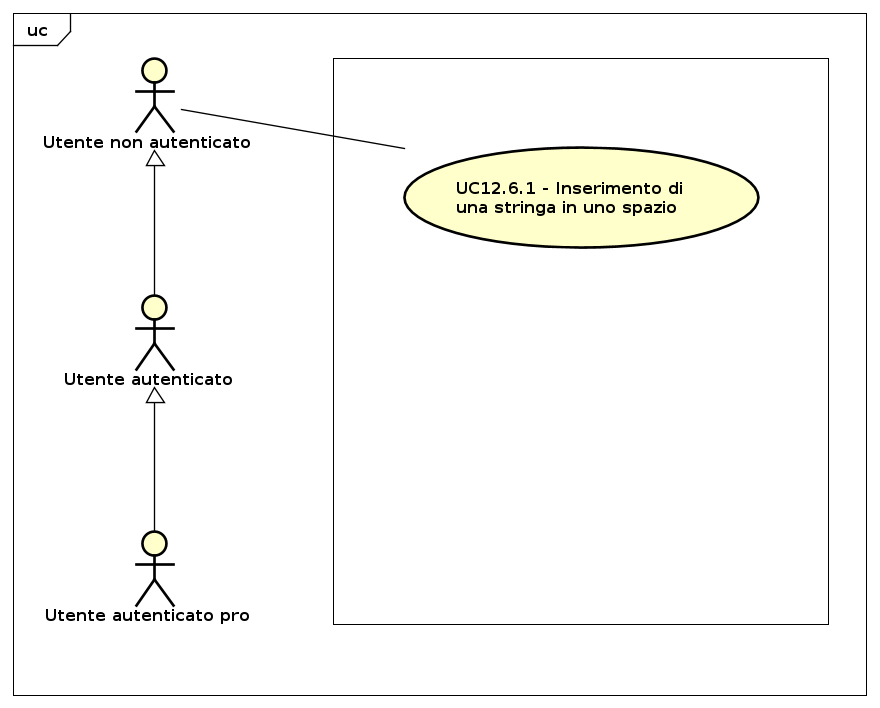
\includegraphics[scale=0.5]{UML/UC12_6.png}
	\caption{UC12.6: Ordinamento di stringhe}
\end{figure}
\begin{itemize}
\item \textbf{Attori}: utente autenticato, utente autenticato pro;
\item \textbf{Descrizione}: l'attore può ordinare le stringhe secondo il criterio richiesto nella domanda inserendole negli appositi spazi;
\item \textbf{Precondizione}: l'attore visualizza la lista non ordinata delle stringhe e la lista vuota in cui andranno inserite;
\item \textbf{Postcondizione}: l'attore ha inserito le stringhe nella lista ordinata;
\item \textbf{Scenario principale}: l'attore ordina le stringhe secondo il criterio richiesto nella domanda inserendole negli appositi spazi (UC12.6.1).
\end{itemize}

\newpage
\paragraph{Caso d'uso UC12.6.1: Inserimento di una stringa in uno spazio}
\begin{figure}[h]
	\centering
	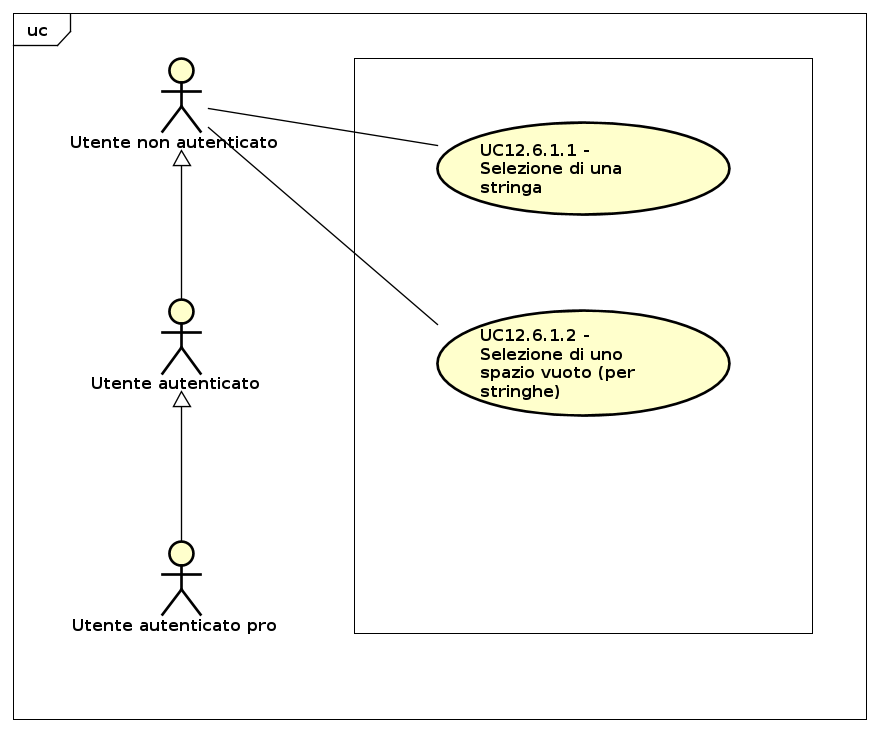
\includegraphics[scale=0.5]{UML/UC12_6_1.png}
	\caption{UC12.6.1: Inserimento di una stringa in uno spazio}
\end{figure}
\begin{itemize}
\item \textbf{Attori}: utente autenticato, utente autenticato pro;
\item \textbf{Descrizione}: l'attore può selezionare una stringa per inserirla in uno spazio vuoto o scambiarla con un'altra se lo spazio è già occupato;
\item \textbf{Precondizione}: l'attore visualizza le stringhe non ordinate e gli spazi vuoti;
\item \textbf{Postcondizione}: l'attore ha inserito la stringa nello spazio selezionato;
\item \textbf{Scenario principale}: l'attore seleziona una stringa (UC12.6.1.1) e la inserisce in uno spazio vuoto o la scambia con un'altra se lo spazio è già occupato (UC12.6.1.2).
\end{itemize}

\subparagraph{Caso d'uso UC12.6.1.1: Selezione di una stringa}
\begin{itemize}
\item \textbf{Attori}: utente autenticato, utente autenticato pro;
\item \textbf{Descrizione}: l'attore può selezionare una stringa;
\item \textbf{Precondizione}: l'attore visualizza le stringhe non ordinate e gli spazi vuoti;
\item \textbf{Postcondizione}: l'attore ha selezionato una stringa;
\item \textbf{Scenario principale}: l'attore seleziona una stringa.
\end{itemize}

\subparagraph{Caso d'uso UC12.6.1.2: Selezione di uno spazio vuoto (per stringhe)}
\begin{itemize}
\item \textbf{Attori}: utente autenticato, utente autenticato pro;
\item \textbf{Descrizione}: l'attore può selezionare uno spazio vuoto;
\item \textbf{Precondizione}: l'attore visualizza le stringhe non ordinate e gli spazi vuoti;
\item \textbf{Postcondizione}: l'attore ha selezionato uno spazio vuoto;
\item \textbf{Scenario principale}: l'attore seleziona uno spazio vuoto.
\end{itemize}

\subsubsection{Caso d'uso UC12.7: Risposta ad una domanda con area cliccabile}
\begin{figure}[h]
	\centering
	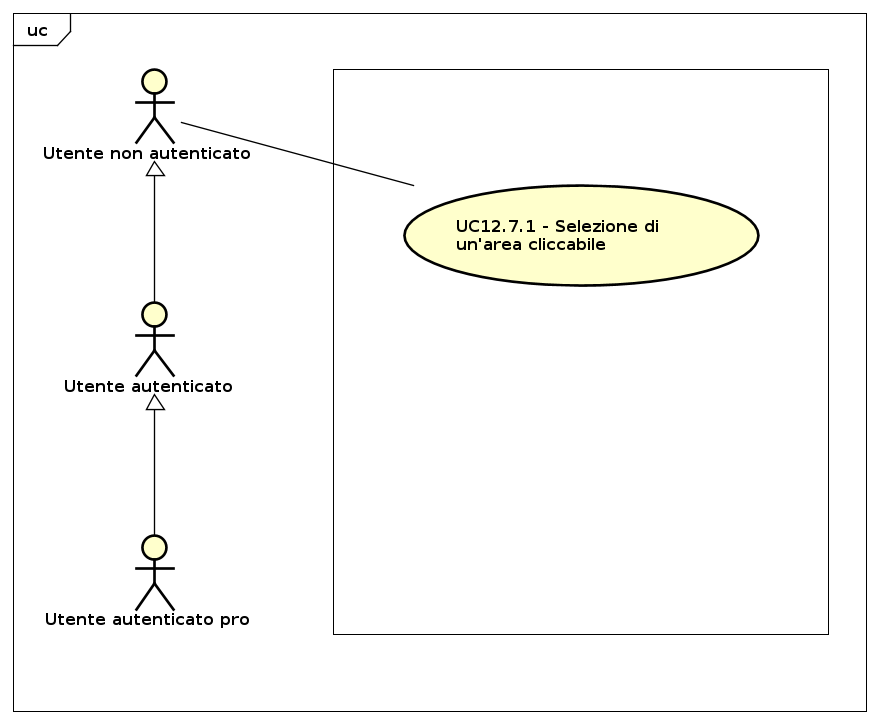
\includegraphics[scale=0.5]{UML/UC12_7.png}
	\caption{UC12.7: Risposta ad una domanda con area cliccabile}
\end{figure}
\begin{itemize}
\item \textbf{Attori}: utente autenticato, utente autenticato pro;
\item \textbf{Descrizione}: l'attore può selezionare una o più aree cliccabili;
\item \textbf{Precondizione}: l'attore visualizza la domanda con area cliccabile;
\item \textbf{Postcondizione}: l'attore ha risposto alla domanda con area cliccabile;
\item \textbf{Scenario principale}: l'attore seleziona una o più aree cliccabili (UC12.7.1).
\end{itemize}

\paragraph{Caso d'uso UC12.7.1: Selezione di un'area cliccabile}
\begin{itemize}
\item \textbf{Attori}: utente autenticato, utente autenticato pro;
\item \textbf{Descrizione}: l'attore può selezionare un'area cliccabile;
\item \textbf{Precondizione}: l'attore visualizza le aree cliccabili;
\item \textbf{Postcondizione}: l'attore ha selezionato un'area cliccabile;
\item \textbf{Scenario principale}: l'attore seleziona un'area cliccabile.
\end{itemize}